%% (Master) Thesis template
% Template version used: v1.4
%
% Largely adapted from Adrian Nievergelt's template for the ADPS
% (lecture notes) project.


%% We use the memoir class because it offers a many easy to use features.
\documentclass[11pt,a4paper,titlepage]{memoir}

%% Packages
%% ========

%% LaTeX Font encoding -- DO NOT CHANGE
\usepackage[OT1]{fontenc}

%% Babel provides support for languages.  'english' uses British
%% English hyphenation and text snippets like "Figure" and
%% "Theorem". Use the option 'ngerman' if your document is in German.
%% Use 'american' for American English.  Note that if you change this,
%% the next LaTeX run may show spurious errors.  Simply run it again.
%% If they persist, remove the .aux file and try again.
\usepackage[english]{babel}

%% Input encoding 'utf8'. In some cases you might need 'utf8x' for
%% extra symbols. Not all editors, especially on Windows, are UTF-8
%% capable, so you may want to use 'latin1' instead.
\usepackage[utf8]{inputenc}

%% This changes default fonts for both text and math mode to use Herman Zapfs
%% excellent Palatino font.  Do not change this.
\usepackage[sc]{mathpazo}

%% The AMS-LaTeX extensions for mathematical typesetting.  Do not
%% remove.
\usepackage{amsmath,amssymb,amsfonts,mathrsfs}

%% NTheorem is a reimplementation of the AMS Theorem package. This
%% will allow us to typeset theorems like examples, proofs and
%% similar.  Do not remove.
%% NOTE: Must be loaded AFTER amsmath, or the \qed placement will
%% break
\usepackage[amsmath,thmmarks]{ntheorem}

%% LaTeX' own graphics handling
\usepackage{graphicx}

%% We unfortunately need this for the Rules chapter.  Remove it
%% afterwards; or at least NEVER use its underlining features.
\usepackage{soul}

%% This allows you to add .pdf files. It is used to add the
%% declaration of originality.
\usepackage{pdfpages}
\usepackage{todonotes}
\usepackage{multirow}

%% MOI: my packages
\usepackage{lmodern}

%% Some more packages that you may want to use.  Have a look at the
%% file, and consult the package docs for each.
%% See the TeXed file for more explanations

%% [OPT] Multi-rowed cells in tabulars
%\usepackage{multirow}

%% [REC] Intelligent cross reference package. This allows for nice
%% combined references that include the reference and a hint to where
%% to look for it.
\usepackage{varioref}

%% [OPT] Easily changeable quotes with \enquote{Text}
%\usepackage[german=swiss]{csquotes}

%% [REC] Format dates and time depending on locale
\usepackage{datetime}

%% [OPT] Provides a \cancel{} command to stroke through mathematics.
%\usepackage{cancel}

%% [NEED] This allows for additional typesetting tools in mathmode.
%% See its excellent documentation.
\usepackage{mathtools}

%% [ADV] Conditional commands
%\usepackage{ifthen}

%% [OPT] Manual large braces or other delimiters.
%\usepackage{bigdelim, bigstrut}

%% [REC] Alternate vector arrows. Use the command \vv{} to get scaled
%% vector arrows.
\usepackage[h]{esvect}

%% [NEED] Some extensions to tabulars and array environments.
\usepackage{array}

%% [OPT] Postscript support via pstricks graphics package. Very
%% diverse applications.
%\usepackage{pstricks,pst-all}

%% [?] This seems to allow us to define some additional counters.
%\usepackage{etex}

%% [ADV] XY-Pic to typeset some matrix-style graphics
%\usepackage[all]{xy}

%% [OPT] This is needed to generate an index at the end of the
%% document.
%\usepackage{makeidx}

%% [OPT] Fancy package for source code listings.  The template text
%% needs it for some LaTeX snippets; remove/adapt the \lstset when you
%% remove the template content.
\usepackage{listings}
\lstset{language=TeX,basicstyle={\normalfont\ttfamily}}

%% [REC] Fancy character protrusion.  Must be loaded after all fonts.
\usepackage[activate]{pdfcprot}

%% [REC] Nicer tables.  Read the excellent documentation.
\usepackage{booktabs}


%% Our layout configuration.  DO NOT CHANGE.
%% Memoir layout setup

%% NOTE: You are strongly advised not to change any of them unless you
%% know what you are doing.  These settings strongly interact in the
%% final look of the document.

% Dependencies
\usepackage{ETHlogo}

% Turn extra space before chapter headings off.
\setlength{\beforechapskip}{0pt}

\nonzeroparskip
\parindent=0pt
\defaultlists

% Chapter style redefinition
\makeatletter

\if@twoside
  \pagestyle{Ruled}
  \copypagestyle{chapter}{Ruled}
\else
  \pagestyle{ruled}
  \copypagestyle{chapter}{ruled}
\fi
\makeoddhead{chapter}{}{}{}
\makeevenhead{chapter}{}{}{}
\makeheadrule{chapter}{\textwidth}{0pt}
\copypagestyle{abstract}{empty}

\makechapterstyle{bianchimod}{%
  \chapterstyle{default}
  \renewcommand*{\chapnamefont}{\normalfont\Large\sffamily}
  \renewcommand*{\chapnumfont}{\normalfont\Large\sffamily}
  \renewcommand*{\printchaptername}{%
    \chapnamefont\centering\@chapapp}
  \renewcommand*{\printchapternum}{\chapnumfont {\thechapter}}
  \renewcommand*{\chaptitlefont}{\normalfont\huge\sffamily}
  \renewcommand*{\printchaptertitle}[1]{%
    \hrule\vskip\onelineskip \centering \chaptitlefont\textbf{\vphantom{gyM}##1}\par}
  \renewcommand*{\afterchaptertitle}{\vskip\onelineskip \hrule\vskip
    \afterchapskip}
  \renewcommand*{\printchapternonum}{%
    \vphantom{\chapnumfont {9}}\afterchapternum}}

% Use the newly defined style
\chapterstyle{bianchimod}

\setsecheadstyle{\Large\bfseries\sffamily}
\setsubsecheadstyle{\large\bfseries\sffamily}
\setsubsubsecheadstyle{\bfseries\sffamily}
\setparaheadstyle{\normalsize\bfseries\sffamily}
\setsubparaheadstyle{\normalsize\itshape\sffamily}
\setsubparaindent{0pt}

% Set captions to a more separated style for clearness
\captionnamefont{\sffamily\bfseries\footnotesize}
\captiontitlefont{\sffamily\footnotesize}
\setlength{\intextsep}{16pt}
\setlength{\belowcaptionskip}{1pt}

% Set section and TOC numbering depth to subsection
\setsecnumdepth{subsection}
\settocdepth{subsection}

%% Titlepage adjustments
\pretitle{\vspace{0pt plus 0.7fill}\begin{center}\HUGE\sffamily\bfseries}
\posttitle{\end{center}\par}
\preauthor{\par\begin{center}\let\and\\\Large\sffamily}
\postauthor{\end{center}}
\predate{\par\begin{center}\Large\sffamily}
\postdate{\end{center}}

\def\@advisors{}
\newcommand{\advisors}[1]{\def\@advisors{#1}}
\def\@department{}
\newcommand{\department}[1]{\def\@department{#1}}
\def\@thesistype{}
\newcommand{\thesistype}[1]{\def\@thesistype{#1}}

\renewcommand{\maketitlehooka}{\noindent\ETHlogo[2in]}

\renewcommand{\maketitlehookb}{\vspace{1in}%
  \par\begin{center}\Large\sffamily\@thesistype\end{center}}

\renewcommand{\maketitlehookd}{%
  \vfill\par
  \begin{flushright}
    \sffamily
    \@advisors\par
    \@department, ETH Z\"urich
  \end{flushright}
}

\checkandfixthelayout

\setlength{\droptitle}{-48pt}

\makeatother

% This defines how theorems should look. Best leave as is.
\theoremstyle{plain}
\setlength\theorempostskipamount{0pt}

%%% Local Variables:
%%% mode: latex
%%% TeX-master: "thesis"
%%% End:


%% Theorem environments.  You will have to adapt this for a German
%% thesis.
%% Theorem-like environments

%% This can be changed according to language. You can comment out the ones you
%% don't need.

\numberwithin{equation}{chapter}

%% German theorems
%\newtheorem{satz}{Satz}[chapter]
%\newtheorem{beispiel}[satz]{Beispiel}
%\newtheorem{bemerkung}[satz]{Bemerkung}
%\newtheorem{korrolar}[satz]{Korrolar}
%\newtheorem{definition}[satz]{Definition}
%\newtheorem{lemma}[satz]{Lemma}
%\newtheorem{proposition}[satz]{Proposition}

%% English variants
\newtheorem{theorem}{Theorem}[chapter]
\newtheorem{example}[theorem]{Example}
\newtheorem{remark}[theorem]{Remark}
\newtheorem{corollary}[theorem]{Corollary}
\newtheorem{definition}[theorem]{Definition}
\newtheorem{lemma}[theorem]{Lemma}
\newtheorem{proposition}[theorem]{Proposition}

%% Proof environment with a small square as a "qed" symbol
\theoremstyle{nonumberplain}
\theorembodyfont{\normalfont}
\theoremsymbol{\ensuremath{\square}}
\newtheorem{proof}{Proof}
%\newtheorem{beweis}{Beweis}


%% Helpful macros.
%% Custom commands
%% ===============

%% Special characters for number sets, e.g. real or complex numbers.
\newcommand{\C}{\mathbb{C}}
\newcommand{\K}{\mathbb{K}}
\newcommand{\N}{\mathbb{N}}
\newcommand{\Q}{\mathbb{Q}}
\newcommand{\R}{\mathbb{R}}
\newcommand{\Z}{\mathbb{Z}}
\newcommand{\X}{\mathbb{X}}

%% Fixed/scaling delimiter examples (see mathtools documentation)
\DeclarePairedDelimiter\abs{\lvert}{\rvert}
\DeclarePairedDelimiter\norm{\lVert}{\rVert}

%% Use the alternative epsilon per default and define the old one as \oldepsilon
\let\oldepsilon\epsilon
\renewcommand{\epsilon}{\ensuremath\varepsilon}

%% Also set the alternate phi as default.
\let\oldphi\phi
\renewcommand{\phi}{\ensuremath{\varphi}}


%% Make document internal hyperlinks wherever possible. (TOC, references)
%% This MUST be loaded after varioref, which is loaded in 'extrapackages'
%% above.  We just load it last to be safe.
\usepackage[linkcolor=black,colorlinks=true,citecolor=black,filecolor=black]{hyperref}


%% Document information
%% ====================

\title{Broad Discourse Context for Language Modeling}
\author{Moisés Torres}
\thesistype{Master Thesis}
\advisors{\textbf{Supervisor:}\\ Prof.\ Dr.\ Thomas Hofmann\\ \hfill \break \textbf{Co-supervisors:}\\ Florian Schmidt\\ Paulina Grnarova}
\department{\hfill \break Department of Computer Science}
\date{November 1, 2017}

\begin{document}

\frontmatter

%% Title page is autogenerated from document information above.  DO
%% NOT CHANGE.
\begin{titlingpage}
  \calccentering{\unitlength}
  \begin{adjustwidth*}{\unitlength-24pt}{-\unitlength-24pt}
    \maketitle
  \end{adjustwidth*}
\end{titlingpage}

%% The abstract of your thesis.  Edit the file as needed.
\begin{abstract}
	
Recurrent neural network language models (RNNLM) have become a key element for state-of-the-art language modeling and are integral parts in a wide range of applications such as speech recognition or information retrieval systems. However, recent attempts have revealed the lack of genuine understanding of standard language models. In particular, the LAMBADA dataset consists of a collection of hard word prediction examples that require to keep track of information in the broader discourse. 

In this thesis we delve into the nature of LAMBADA and highlight the impact that rare words have on the overall results. We introduce our proposed model, the Softmax Mixture, and showcase through a series of experiments its ability to handle rare words when compared to vanilla RNNLMs. We further implement the Pointer Sentinel Mixture model and demonstrate that it achieves perplexities on par with the state-of-the-art on LAMBADA while having superior adaptation capabilities.

\noindent\textbf{Keywords:} language modeling, recurrent neural networks (RNN), LAMBADA dataset, rare word problem, pointer models.
 
\end{abstract}

\cleardoublepage

%%MOI: Add acknowledgments
\renewcommand{\abstractname}{Acknowledgments}
\begin{abstract}
	
First, I want to thank my supervisor, Prof.Thomas Hofmann, for allowing me to do my thesis in the Data Analytics laboratory. I am also thankful for his	early comments that helped steering the project in the right direction.
	
I would like to express my gratitude to Florian Schmidt and Paulina Grnarova for providing me such an interesting and challenging thesis topic. I further thank them for the insightful discussions that we had all along the project and for helping me proofreading this report.
  
I thank all my friends that made me think of Zurich as a second home.
  
Finally, I would like to thank my family and specially my parents. Without your unconditional support I would not be writing this thanking words in the first place.
\end{abstract}

\cleardoublepage

%% TOC with the proper setup, do not change.
\cleartorecto
\tableofcontents
\mainmatter

%% Your real content!
\chapter{Introduction}

Probabilistic language modeling is the area of Natural Language Processing (NLP) concerned with the development of statistical models capable of assigning probabilities over sequences of words $p(w_1, \ldots ,w_n)$. Such models are of great use in applications like automatic speech recognition, where the uncertainty of choosing among sentences with very similar pronunciation profiles can be reduced by explicitly modeling how likely is each word sequence. Another example are dialogue systems, where discourse understanding is needed to produce valid utterances for a given conversation context. Currently, recurrent neural network based language models hold the state-of-the-art.

\section{Problem Statement and Motivation}
\label{sec:motivation} 

Recent works like \cite{paperno2016lambada} and \cite{jia2017adversarial} have highlighted that in spite of the good performances achieved under standard metrics, modern models are far from genuine language understanding. This is mostly due to the fact that current evaluation methodologies fail at probing the actual capabilities of these models. In particular, examples like the LAMBADA dataset, have shown that SOTA language models fail to take the broad discourse context into account when predicting a word.

Moreover, further research efforts like \cite{merity2016pointer} suggest that in general, existing neural language models have the fundamental problem of failing to handle rare words. Despite its limited effect on the overall perplexity, rare word prediction is a significant issue for language models. This problem becomes very important in applications that rely on knowledge-extraction, such as question-answering or reading comprehension, where rare words are of primary interest.

\section{Thesis Contributions}
\label{sec:contribution}

The main contributions of this thesis can be summarized as follows:

\begin{itemize}

\item We study the nature of the LAMBADA dataset and the phenomena that contribute to its difficulty. We also perform an extensive analysis of its main characteristics and use those findings to motivate the subsequently proposed approaches. 

\item We present our model, the Softmax Mixture, which attempts to separately model the output distribution of rare words by introducing an additional softmax layer. By dynamically calculating the weight of the two distributions, our objective is that the model learns which one to use depending on the history of previous words.

\item We test the behavior of the Softmax Mixture under multiple configurations and analyze the impact of the switching component in the overall performance of the model.

\item We apply a variant of a pointer based language model to the LAMBADA task and perform a quantitative and qualitative analysis of the results.

\end{itemize}

\section{Thesis Outline}
\label{sec:outline}

The remainder of this thesis is organized in the following way:

\begin{itemize}

\item In Chapter 2 we give an overview of the related work, mainly focusing on recurrent neural network language models and recently proposed extensions.

\item Chapter 3 starts by introducing the basics of language modeling. We then review the development of neural language models and their main weaknesses, detailing how they have been addressed in the literature.

\item The LAMBADA dataset is presented in Chapter 4 together with a detailed analysis of its main characteristics. We proceed to discuss the rare word problem and how it applies to LAMBADA and conclude with the examination of several RNN regularization techniques.

\item Chapter 5 compares several recently proposed architectures designed to extend vanilla RNNLMs and tackle the rare word prediction problem. We also introduce our proposed model called the ``Softmax Mixture''.

\item The experiments carried out in this thesis are detailed in Chapter 6. We first discuss the behavior shown by different configurations of the Softmax Mixture model and then we further analyze the cause for the obtained performance. Additionally, we apply to Pointer Sentinel Mixture model to the LAMBADA task and comment on the results.

\item Finally we present our conclusions and discuss prospective future work directions in Chapter 7.

\end{itemize}

\chapter{Related Work}

This chapter gives a brief overview of the state-of-the-art techniques used for word-level neural language modeling.

Recurrent neural network language models (RNNLM) \cite{mikolov2010recurrent} introduced by Mikolov et al. (2010) have become ubiquitous in modern language modeling. RNNLMs incorporate the advantages of previous attempts at neural language modeling \cite{bengio2003neural}, namely projecting words into low dimensional space solving smoothing implicitly and being trained with standard backpropagation techniques. In addition to that, recurrent networks have the ability to learn how to compress arbitrary long histories into low dimensional space. Jozefowicz et al. (2016) explored the performance gains achieved by these architectures when trained on large scale datasets \cite{jozefowicz2016exploring}.

Several improvements have since then been proposed to improve on vanilla RNNLMs:

Kim et al. (2015) introduced a novel method that only relies on character-level information to predict words, which is specially helpful for morphologically rich languages \cite{kim2016character}. Word characters are processed by a one-dimensional convolutional layer and fed through a highway network in order to obtain the word representations. Despite requiring fewer parameters, character-aware models are on par with their word-level counterparts.

On a different note, using large vocabularies can be sometimes unfeasible as calculating the output probability of a word implies computing the whole distribution due to the normalization necessary for the softmax operation, which makes training prohibitively slow. Mnih \& Hinton (2009) employ a hierarchical representation of the vocabulary in the form of a binary tree in which the output probability of a word is directly encoded in the path specified by the hierarchy \cite{mnih2009scalable}. Another possible approach relies on Noise Contrastive Estimation (NCE), which introduces a surrogate binary classification task in which a classifier is trained to discriminate between the true data and samples coming from a noise distribution \cite{mnih2012fast}. In both cases normalization is rendered unnecessary, which makes this techniques specially appealing for large scale models.

Regarding regularization, Zaremba et al. (2014) was one of the first to successfully apply dropout to RNNs \cite{zaremba2014recurrent}. A random binary mask is only applied to the non-recurrent connections, the cell's inputs and outputs. In \cite{gal2016theoretically}, Gal \& Ghahramani (2016) provide a bayesian interpretation for dropout (known as variational dropout) and use it to argue that the mask should be the same for all time steps and also applied to the recurrent connections. A different approach called zoneout is taken by Krueger et al. (2016) in \cite{krueger2016zoneout}, where randomly selected neurons of the hidden state are not updated (in contrast with being dropped). More recently Merity et al. (2017) introduced another regularization variant where dropout is applied to the hidden-to-hidden recurrent weights rather than directly to the hidden states. In combination with other techniques, this method has achieved state-of-the-art perplexities on several datasets \cite{merity2017regularizing}.

Following the work in deep RNNs, recurrent highway networks (RHN) \cite{zilly2016recurrent} introduced by Zilly et al. (2016) extend LSTMs to enable the learning of deep recurrent state transitions. This is achieved by modifying the LSTM cell to allow multiple hidden state updates per time step.

Inan et al. (2016) make a case for sharing the weights between the embeddings and the softmax layer \cite{inan2016tying}, which improves previous results and significantly reduces the amount of trainable parameters. This technique is theoretically motivated and takes advantage of the metric encoded into the space of word embeddings to generate a more informed target distribution. This prevents the model from having to learn a one-to-one correspondence between the input and output.

Similar to other areas of NLP, several memory augmented architectures have been proposed for language modeling. Daniluk et al. (2017) formulate an attention mechanism for RNNLMs \cite{daniluk2017frustratingly} and explores to what extent is the learning of long-range dependencies improved. Grave et al. (2016) and Merity et. al (2016) proposed pointer based attention models where a probability distribution is generated over the history of recent words and blended with the distribution over the whole vocabulary. While the former doesn't need to be trained \cite{grave2016improving}, the latter introduces additional parametrization that allows to calculate the interpolation weight of the two distributions dynamically \cite{merity2016pointer}.

A very interesting research direction has been recently proposed by Zoph \& Le (2016), where a reinforcement learning agent is used to generate custom
RNN cell architectures tailored to the specific task of language modeling \cite{zoph2016neural}.

With respect to the evaluation of RNNLMs, Melis et al. (2017) stress the importance of careful hyperparemeter tuning and arrive at the conclussion that standard LSTM architectures, when properly regularised, outperform more recent models \cite{melis2017state}. Paperno et al. (2016) raise their concerns with regards to the genuine language understanding of SOTA models and introduce LAMBADA \cite{paperno2016lambada}, a dataset specifically designed to put this to the test. Along these lines, Jia \& Liang (2017) propose a method to build adversarial examples for reading comprehension systems and find out that when evaluated on them, models produce very poor results under standard evaluation metrics \cite{jia2017adversarial}.
\chapter{Neural Language Models}

In this chapter, we introduce the notation used throughout the thesis and give a brief overview of the development of neural language models (NLM). We also review some of the main weaknesses shown by this family of models and how they have been addressed in the literature. 

\todo{
	- Finish this (7-8 pages) \\
	- Mention CNN LMs ? \\
	- Softmax variants (hierarchical)? \\
	- Modern models (highway)? \\
	- Include references for n-grams? \\
	- Should I create my own figures?
}

\section{Notation}
\label{sec:notation}

Before continuing, we will define the notation used in the thesis:

\begin{itemize}
	\item Scalars are denoted with lowercase letters, such as $x$.
	
	\item Vectors are denoted with bold lowercase letters, such as $\mathbf{x}$ with $\mathbf{x}_i$ its $i$-th element, and are always assumed to be column vectors.
	
	\item Matrices are denoted with uppercase letters, such as $X$ with $X_{ij}$ as its $(i,j)$-th element.
\end{itemize}

\section{Background}
\label{sec:background}

Prior to introducing the specifics of NLMs, we will formalize the task at hand and introduce some of its core concepts. 

\subsection{Language Modeling}

First, we define a \textbf{word-based language model} as a model able to compute the probability of a sentence or sequence of words $p(w_1, \ldots ,w_n)$. Such models are of great use in tasks where we have to recognize words in noisy or ambiguous input such as speech recognition or machine translation, among others.

If we now decompose the joint probability of a sequence using the chain rule of probability as shown in \autoref{eq:lm}, we observe that the function that needs to be estimated boils down to the conditional probability of a word given the history of previous words. However, taking into account the whole context poses a problem as language is creative and any particular sequence might have occurred few (or no) times before.  Many of the models that we will introduce approximate the true conditional distribution by making a Markov assumption as shown in \autoref{eq:markov}. This means that the probability of an upcoming word is fully characterized by the previous $n-1$ words. Despite seeming an incorrect premise for a complex source of information such as language, it has been proven to work really well in practice.

\begin{equation} \label{eq:lm}
	\begin{gathered}
		p(w_1, \ldots ,w_n)=p(w_1)p(w_2|w_1)p(w_3|w_{1}^{2}) \ldots p(w_n|w_{1}^{n-1}) \\
		= \prod_{k=1}^{n} p(w_k|w_{1}^{k-1})
	\end{gathered}
\end{equation}

\begin{equation} \label{eq:markov}
	p(w_k|w_{1}^{k-1}) \approx p(w_k|w_{k-1}^{k-n})
\end{equation}

\subsection{Evaluation}

Following a common practice in machine learning, we use a test set in order to evaluate our models. In the case of language modeling we have a word sequence $W_1^n=\{w_1, \ldots , w_n\}$ and we expect the model to assign it a high probability. Rather than working directly with raw probabilities we define a metric called \textbf{perplexity}, which is the geometric average of the inverse of the probability over the test set, as shown in \autoref{eq:pp}. Therefore, lower perplexity is better.

\begin{equation} \label{eq:pp}
	\begin{gathered}
		\text{Perplexity}(W_1^n) = p(W_1^n)^{-\frac{1}{n}} = \sqrt[n]{\frac{1}{p(W_1^n)}} \\
		= \sqrt[n]{\frac{1}{\prod_{k=1}^{n} p(w_k|W_{1}^{k-1})}}
	\end{gathered}
\end{equation}

Moreover, we can regard language as an information source and therefore use Information Theory to find a different (and equivalent) interpretation of perplexity. For that we need to introduce the basic concept of \textbf{entropy} (\autoref{eq:entropy} shows its formulation for discrete variables), which measures the expected uncertainty or ``surprise" $S$ of the value of a random variable $X$. Without going into details, it is easy to see that defining uncertainty as the negative logarithm (the specific base doesn't matter, but traditionally it is assumed to be 2) of the probability of each event matches our intuition (like $S(p)>S(q) \ \text{then} \ p<q$).

\begin{equation} \label{eq:entropy}
	H(X)=\mathbb{E}[S(X)]=-\sum_{x \in \mathcal{X}}p(x)\log_2(p(x)) \quad \text{with} \quad S(\cdot)=-\log_2(\cdot)
\end{equation}

A difference when it comes to language is that it involves dealing with sequences $W_1^n$ of discrete random variables. For a given language $L$ we can define the entropy of a variable ranging over all possible sequences of length $n$. To obtain the entropy-per-word we only need to normalize by $n$ (\autoref{eq:entropySeq}).

\begin{equation} \label{eq:entropySeq}
	\frac{1}{n} H(W_1^n) = -\frac{1}{n}\sum_{W_1^n \in L}p(W_1^n)\log_2(p(W_1^n))
\end{equation}

Additionally, in order to calculate the true entropy of a language we would need to consider sequences of infinite length (\autoref{eq:trueEntropySeq}). Fortunately, the Shannon-McMillan-Breiman theorem states that if a stochastic source (such as language) is regular in certain ways (stationary and ergodic) we can take a single long enough sequence instead of summing over all possible sequences (* in \autoref{eq:trueEntropySeq}).

\begin{equation} \label{eq:trueEntropySeq}
	\begin{gathered}
		H(L) = -\lim\limits_{n \rightarrow \infty}\frac{1}{n}\sum_{W_1^n \in L}p(W_1^n)\log_2(p(W_1^n))\\
		\stackrel{*}{=} -\lim\limits_{n \rightarrow \infty}\frac{1}{n}\log_2(p(W_1^n))
	\end{gathered}
\end{equation}

Related to the concept of entropy we have \textbf{cross-entropy}, which measures the relative entropy of $p$ with respect to $m$, $p$ being the true probability distribution and $m$ a model (e.g. an approximation) of $p$ over the same underlying set of events. After applying the Shannon-McMillan-Breiman theorem and assuming that $n$ is large enough, we can see in \autoref{eq:crossEntropy} the final formulation of the cross-entropy, which has become the standard loss function when optimizing neural language models.

\begin{equation} \label{eq:crossEntropy}
	\begin{gathered}
		H(p,m) = -\lim\limits_{n \rightarrow \infty}\frac{1}{n}\sum_{W_1^n \in L}p(W_1^n)\log_2(m(W_1^n)) \\
		\stackrel{*}{=} -\lim\limits_{n \rightarrow \infty}\frac{1}{n}\log_2(m(W_1^n)) \approx -\frac{1}{n}\log_2(m(W_1^n)) \\
		= -\frac{1}{n}\sum_{k=1}^{n}\log_2(m(w_k|W_{1}^{k-1}))
	\end{gathered}
\end{equation}

Finally, we can see in \autoref{eq:relationCrossAndPP} how cross-entropy and perplexity are connected. This relation gives raise to a nice interpretation of perplexity as branching factor: entropy measures uncertainty (in bits, if we use $\log_2$) but in exponentiated form it is measured as the cardinality of a uniform distribution with equivalent uncertainty.

\begin{equation} \label{eq:relationCrossAndPP}
	\text{Perplexity}(W_1^n) = 2^{H(p,m)} = m(W_1^n)^{-\frac{1}{n}}
\end{equation}

\section{Feed-Forward Neural Language Models (FFNLM)}
\label{sec:forwardnlm}

Until the appearance of NLMs, the most successful approaches were based on n-grams, which are models that estimate words from a fixed window of previous words and estimate probabilities by counting in a corpus and normalizing. Due to their nature, n-gram estimates intrinsically suffer from sparsity and several methods like smoothing, backoff and interpolation have been proposed to deal with this problem \cite{chen1996empirical}.

Along those lines, the first successful attempt of applying neural networks to language modeling \cite{bengio2003neural} remarked the effect of the \textit{curse of dimensionality} when it comes to estimating the joint distribution of many discrete random variables (such as words in a sentence). On the contrary, by using continuous variables we obtain better generalization because the function to be learned can be expected to have some local smoothness properties (``similar" words should get similar probabilities of being predicted). While requiring to be trained (n-grams don't), this approach is able to achieve significantly better results (reductions between 10\% and 20\% in perplexity with respect to a smoothed trigram model) by jointly learning word representations and a statistical language model.

Similar to n-grams, the model introduced in \cite{bengio2003neural} conditions the probability of a word on the previous $n-1$ words. The main difference lies in the concept of \textbf{distributed feature vectors}; words are embedded into a vector-space by assigning them a real vector representation of size $m$ via a look-up operation over the embedding matrix $C$ as shown in \autoref{eq:fwnlm}. 

\begin{equation} \label{eq:fwnlm}
	\begin{gathered}
		\mathbf{x} = [C_{w_{t-1},:} \, , C_{w_{t-2},:} \, , \cdots \, , C_{w_{t-n+1},:})] \\
		\mathbf{y} = W\mathbf{x} + U \tanh(H\mathbf{x}+\mathbf{d}) + \mathbf{b} \\
		\hat{p}(w_t=i|w_{t-1},\ldots,w_{t-n+1}) = \frac{e^{\mathbf{y}_i}}{\sum_{n}e^{\mathbf{y}_n}} \\
	\end{gathered}
\end{equation}

where $C \in \mathbb{R}^{|V| \times m}$, $\mathbf{x} \in \mathbb{R}^{1 \times (n-1)m}$, $W \in \mathbb{R}^{|V| \times (n-1)m}$, $U \in \mathbb{R}^{|V| \times h}$, $H \in \mathbb{R}^{h \times (n-1)m}$, $\mathbf{d} \in \mathbb{R}^{h}$ and $\mathbf{y} ,\mathbf{b} \in \mathbb{R}^{|V|}$. The concatenated word representations $\mathbf{x}$ are fed through one (or more) nonlinear hidden layer (weights $H$ and bias $\mathbf{d}$), resulting in a hidden representation of size $h$. We then apply an affine transformation (weights $U$ and bias $\mathbf{b}$) to this hidden representation to obtain $\mathbf{y}$, an unnormalized probability distribution over the vocabulary $V$. Optionally, we can include direct connections from the word features to the output ($W$). Finally, a softmax operation produces a valid probability distribution over the full vocabulary.

\begin{figure}[H]
	\centering
	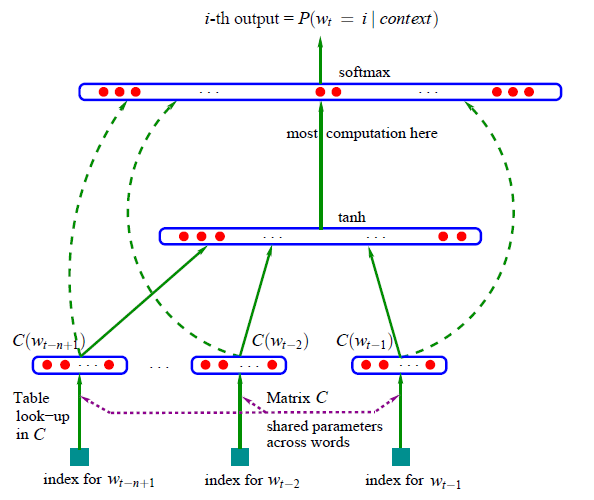
\includegraphics[scale=0.5]{fflm}
	\captionof{figure}{Feed-Forward NLM architecture \cite{bengio2003neural}}
	\label{fig:ffarch}
\end{figure}

Having a look at the full model (shown in \autoref{fig:ffarch}) we can observe that most expensive operation is the computation of the unnormalized probability distribution $\mathbf{y}$, which requires a number of dot products that scales linearly with $|V|$ (it is not unusual to work with vocabulary sizes in the order of the tens of thousands). 

Several practical solutions have been proposed to avoid it, with \textbf{hierarchical softmax} \cite{morin2005hierarchical} being one of the most popular ones. It uses a hierarchical binary tree representation of the vocabulary with words as
its leaves and, for each node, explicitly represents the relative probabilities of its child nodes. These define a random walk that assigns probabilities to words, allowing to reduce the complexity of obtaining the output probability of a single word to around $\log_2(|V|)$.

\section{Word Vectors}
\label{sec:wv}

As we stated in the previous section, distributed continuous vectors allow for ``clever" smoothing by taking into account syntactic and semantic features that are automatically learnt. \cite{mikolov2013efficient} picked up on this concept trying to find ways of training these vector representations more efficiently. The paper introduces a family of models known as \textbf{word2vec}, whose architecture matches the one from a FFNLM where the nonlinear hidden layer has been removed (ending up with a simple log bilinear model). The difference between them lies on the objective they optimize for. It is important to note that these objectives are designed as a mean to learn meaningful word embeddings, which are the main focus of the following architectures:

\begin{itemize}
	\item Continuous Bag-of-Words model (CBOW): given a symmetric window of size $k$ around a specific position $i$ $\{w_{i-k}, \ldots , w_{i-1}, w_{i+1}, \ldots w_{i+k}\}$, we want to predict the word $w_i$. The term ``bag-of-words" comes from the fact that the embeddings of the whole window are summed (instead of concatenated) and thus, order is not preserved.
	
	\item Continuous Skip-Gram model: given a specific position $i$ we randomly sample words inside its surrounding window and try to predict them. Therefore, each training example is a 2-tuple consisting of $w_i$ as input and a sampled word from the window as output.
\end{itemize}

In addition to a simplified architecture and a modified objective, further optimizations for the Skip-Gram model were introduced in a follow-up paper \cite{mikolov2013distributed}. As we already explained at the end of the previous section, calculating a probability distribution over the full vocabulary is computation-intensive. In order to avoid doing this, the original task is casted into a binary classification problem by making use of a new objective named \textbf{negative sampling}. Inspired by noise contrastive estimation (NCE), the objective is to distinguish the target word $w_O$ from draws coming from a noise distribution $p_n(w)$ (e.g. unigram distribution) using logistic regression, where there are $k$ noise samples for each data point (\autoref{eq:ns}).

\begin{equation} \label{eq:ns}
	\begin{gathered}
		\mathcal{L}(\theta) = \log(\sigma(\mathbf{v_{w_O}}^{\top} \mathbf{v_{w_I}})) + \sum_{i=1}^{k} \log(-\sigma(\mathbf{v_{w_i}}^{\top} \mathbf{v_{w_I}})) \\ 
		\text{with} \quad w_i \sim p_n(w)
	\end{gathered}
\end{equation}

Another famous family of word vectors is \textbf{GloVe} \cite{pennington2014glove}, where the objective is a weighted (weighting function $f(\cdot)$) least squares fit of the log-counts (\autoref{eq:glove}). Rather than capturing co-occurences one word at a time (like word2vec), GloVe does dimensionality reduction on the whole co-occurrence counts matrix $N$. 

\begin{equation} \label{eq:glove}
	\mathcal{L}(\theta, N) = \sum_{i,j:N_{ij}>0}f(N_{ij})(\log(N_{ij})-(\mathbf{v_{w_O}}^{\top} \mathbf{v_{w_I}} + b_O + b_I))^2
\end{equation}

In general, word vectors have proven to excel at capturing semantic features. For example, \cite{mikolov2013efficient} analyzes how Skip-Gram vectors achieve very good results on the semantic word relationship task. Furthermore, the authors qualitatively explore how the resulting vector representations encode semantic information in the affine embedding structure. Hence, a vector operation like $\textit{Spain}-\textit{Madrid}+\textit{Switzerland}$ would lead to the desired answer $\textit{Bern}$.

In summary, word vectors have become a standard in NLP and are used as input in all sorts of downstream applications such as sentiment analysis.

\section{Recurrent Neural Language Models (RNLM)}
\label{sec:rnn}

So far all the models that we have seen (n-grams and FFNLM) explicitly use a fixed length context. Recurrent neural networks remove this limitation by introducing recurrent connections that allow information to cycle for an arbitrarily long time (although this is not true in practice). They learn to compress the whole history in low dimensional space (hidden state $\mathbf{h}(t)$) that is sequentially updated by being blended with the current input $\mathbf{x}(t)$ (\autoref{eq:rnncell} introduces the formulation for Elman networks).

\begin{equation} \label{eq:rnncell}
		\mathbf{h}(t) = \sigma_h(W_h \mathbf{x}(t) + U_h \mathbf{h}(t-1) + \mathbf{b_h})
\end{equation}

where $W_h \in \mathbb{R}^{h \times m}$, $\mathbf{x}(t) \in \mathbb{R}^{m}$, $U_h \in \mathbb{R}^{h \times h} , \mathbf{h}(t), \mathbf{h}(t-1), \mathbf{b_h} \in \mathbb{R}^{h}$ and $\sigma_h$ is a nonlinear function (e.g. sigmoid). It is important to note that the network parameters are shared over time. \cite{mikolov2010recurrent} was one of the first to successfully apply RNNs to language modeling. The hidden states $\mathbf{h}(t)$ are fed through a fully connected layer to produce a probability distribution over the vocabulary in a similar way to FFNLM.

\begin{equation} \label{eq:rnnlm}
	\begin{gathered}
		\mathbf{y}(t) = W_y \mathbf{h}(t) + \mathbf{b_y} \\
		\hat{p}(w_t=i|\mathbf{h}(t)) = \frac{e^{\mathbf{y}(t)_i}}{\sum_{n}e^{\mathbf{y}(t)_n}} \\
	\end{gathered}
\end{equation}

where $W_y \in \mathbb{R}^{|V| \times h}$ and $\mathbf{y}(t)$, $\mathbf{b_y} \in \mathbb{R}^{|V|}$.

\subsection{Backpropagation Through Time (BPTT)}

Backpropagation is the standard gradient computation technique used for neural networks. However when applied to the recurrent connections of an RNN, the gradients will depend on the previous timesteps (up to $t=0$). Thus, we call Backpropagation Through Time (BPTT) \cite{werbos1990backpropagation} to the application of backpropagation on an unrolled RNN, which accounts for this dependencies by summing up the gradients for each time step. In \autoref{eq:bptt} we see an example of this when calculating the gradient for $U_h$.

\begin{equation} \label{eq:bptt}
\frac{\partial \mathcal{L}(t)}{\partial U_h} = \frac{\partial \mathcal{L}(t)}{\partial \mathbf{\hat{p}}(t)}\frac{\partial \mathbf{\hat{p}}(t)}{\partial \mathbf{h}(t)}\frac{\partial \mathbf{h}(t)}{\partial U_h} = \sum_{k=0}^{t} \frac{\partial \mathcal{L}(t)}{\partial \mathbf{\hat{p}}(t)}\frac{\partial \mathbf{\hat{p}}(t)}{\partial \mathbf{h}(t)}\frac{\partial \mathbf{h}(t)}{\partial \mathbf{h}(k)}\frac{\partial \mathbf{h}(k)}{\partial U_h}
\end{equation}

One of the main problems of BPTT is the high cost of a single parameter update, which makes it impossible to use for large numbers of iterations. \textbf{Truncated Backpropagation Through Time} (TBPTT), which is a modified version of BPTT, was introduced in \cite{sutskever2013training} to work around this limitation. When using TBPTT, the sequence is processed one timestep at a time, and every $k_1$ timesteps, it runs BPTT for $k_2$ timesteps, so a parameter update can be cheap if $k_2$ is small. Most implementations assume $k_1=k_2$.

\subsection{Exploding and Vanishing Gradient}

If input sequences are comprised of thousands of timesteps, then this will be the number of derivatives required for a single weight update. We can see this in \autoref{eq:gradient} by observing that the term $\frac{\partial \mathbf{h}(t)}{\partial \mathbf{h}(k)}$ is a chain-rule itself. Citing \cite{pascanu2013difficulty}, \textit{``a product of $t-k$ real numbers can shrink to zero or explode to infinity, so does this product of matrices"} and therefore, this can cause gradients to vanish or explode. 

\begin{equation} \label{eq:gradient}
	\frac{\partial \mathbf{h}(t)}{\partial \mathbf{h}(k)} = \prod_{t \geq i > k} \frac{\partial \mathbf{h}(i)}{\partial \mathbf{h}(i-1)}
\end{equation}

For exploding gradients, clipping the norm of the gradients to a pre-defined threshold has proven to be an effective remedy for this problem. On the other hand, vanishing gradient translates into gradient contributions from ``far away" steps becoming zero, and thus hindering the learning of long-range dependencies. The most popular solution for this problem has been the introduction of new cell architectures explicitly designed to deal with vanishing gradients such as Long Short-Term Memory (LSTM) \cite{hochreiter1997long} and Gated Recurrent Units (GRU) \cite{cho2014learning}. We will focus on the LSTM as the GRU cell is just a simplified version of the former.

\begin{equation} \label{eq:lstmcell}
	\begin{gathered}
		\mathbf{f}(t) = \sigma_g(W_f \mathbf{h}(t-1) + U_f\mathbf{x}(t) + \mathbf{b}_f) \\
		\mathbf{i}(t) = \sigma_g(W_i \mathbf{h}(t-1) + U_i \mathbf{x}(t) + \mathbf{b}_i) \\
		\mathbf{o}(t) = \sigma_g(W_o \mathbf{h}(t-1) + U_o \mathbf{x}(t) + \mathbf{b}_o) \\
		\mathbf{\tilde{c}}(t) = \sigma_c(W_c \mathbf{h}(t-1) + U_c \mathbf{x}(t) + \mathbf{b}_c) \\
		\mathbf{c}(t) = \mathbf{f}(t) \odot \mathbf{c}(t-1) + \mathbf{i}(t) \odot \mathbf{\tilde{c}}(t) \\
		\mathbf{h}(t) = \mathbf{o}(t) \odot \sigma_h(\mathbf{c}(t))\\
	\end{gathered}
\end{equation}

where $W_f,W_i,W_o,W_f \in \mathbb{R}^{h \times h}$, $U_f,U_i,U_o,U_f \in \mathbb{R}^{h \times m}$, $\mathbf{f}(t),\mathbf{b}_f,\mathbf{i}(t),\mathbf{b}_i,  \allowbreak \mathbf{o}(t),\mathbf{b}_o,\mathbf{c}(t),\mathbf{b}_c,\mathbf{\tilde{c}}(t) \in \mathbb{R}^{h}$ and $\sigma_g,\sigma_c,\sigma_h$ are non linear functions. The main differences to a vanilla RNN are the introduction of a cell state $\mathbf{c}_t$ (that acts as internal memory) and the gates $\mathbf{f}$, $\mathbf{i}$ and $\mathbf{o}$. Gates are a way to optionally let information through and are learnt in such a way that the cell can remember long-range dependencies. As shown in \autoref{eq:lstmcell}, the new cell state is formed by a combination of the previous cell state weighted by the forget gate $\mathbf{f}(t)$ and the ``newly proposed" state $\mathbf{\tilde{c}}(t)$ weighted by the input gate $\mathbf{i}(t)$.

To sum up, recurrent neural network architectures using LSTM cells have become ubiquitous in a wide range of NLP tasks and are a key element in state-of-the-art language models \cite{jozefowicz2016exploring}.

\chapter{Rare Word Prediction}

In this chapter we present the LAMBADA dataset, which will be used throughout this thesis to evaluate our different models. We also discuss the rare word problem and examine several RNN regularization techniques.

\section{The LAMBADA dataset}
\label{sec:lambada}

This dataset was first introduced in \cite{paperno2016lambada} as a challenging test set specifically designed to probe the genuine language understanding of state-of-the-art NLP models. In the authors' words, \textit{``models' effectiveness at picking statistical generalizations from large corpora can lead to the illusion that they are reaching a deeper degree of understanding than they really are''}. Below we can find an example extracted from the dataset:

\begin{figure}[H]
	\begin{mdframed}[linewidth=1pt]
	\begin{quote} 		
		\textbf{Context:} \textit{``Why?'' ``I would have thought you'd find him rather dry,'' she said. ``I don’t know about that,'' said \underline{Gabriel}. ``He was a great craftsman,'' said Heather. ``That he was,'' said Flannery.} \par
		\textbf{Target sentence:} \textit{``And Polish, to boot,'' said $\rule{1.2cm}{0.15mm}$} . \par
		\textbf{Target word:} \textit{Gabriel}
	\end{quote}
	\end{mdframed}
	\caption{Example of a LAMBADA passage} \label{fig:lambadaPassage}
\end{figure}

As illustrated in \autoref{fig:lambadaPassage}, the dataset consists of narrative passages formed by a \textit{context paragraph} (with an average length of 4.6 sentences) and a \textit{target sentence}. The objective is to predict the last word of the target sentence (known as the \textit{target word}). In this way, LAMBADA casts the complex task of evaluating language understanding into the simple and general word prediction framework of language modeling.

\subsection{Construction Process}

LAMBADA was built using a large initial dataset, BookCorpus, which was then distilled into a difficult subset. The original dataset features 5325 unpublished novels (after duplicate removal) and 465 million words \cite{zhu2015aligning}. Novels were then randomly divided into equally-sized training and development+test partitions. Models tackling LAMBADA are intended to be trained on raw text from the training partition, which encompasses 2662 novels and more than 200 million words.

In order to obtain the LAMBADA passages, an automated filtering step was first applied to the development+test partition. In particular, passages from the initial candidate set were discarded if the target word was given a probability $\geq 0.00175$ by any of the four different standard language models (both neural and count based) that were used in this stage of the process.

To make it into the final dataset, the remaining passages were then evaluated by human subjects in a three-step process:

\begin{enumerate}
	\item A human evaluator had to guess the target word correctly based on the whole passage (comprising the context and the target sentence).
	\item A second human evaluator had to also guess the target word correctly in the same conditions.
	\item Finally, ten human evaluators had to fail at guessing the target word having access to only the target sentence and 3 allowed attempts.
\end{enumerate}

Due to the specifics of this process, the passages that finally were selected have the property of not being guessable by just relying on local context and require broader understanding, probing the long range capabilities of language models. The final development and test sets that constitute LAMBADA consist of 4869 and 5153 passages, respectively. Additionally, a control set containing 5000 unfiltered passages was also constructed to allow for comparisons between standard language modeling scenarios and LAMBADA.

\subsection{Dataset Analysis}

The authors theorize that the inspection of the LAMBADA data suggests that, in order for the target word to be predictable in a broad context only (which is the case of LAMBADA by design), it must be strongly cued in the broader discourse. \autoref{fig:lambadaContext} compares the proportion of passages in the LAMBADA and control sets that include the target word in the context.

\begin{figure}[H]
	\centering
	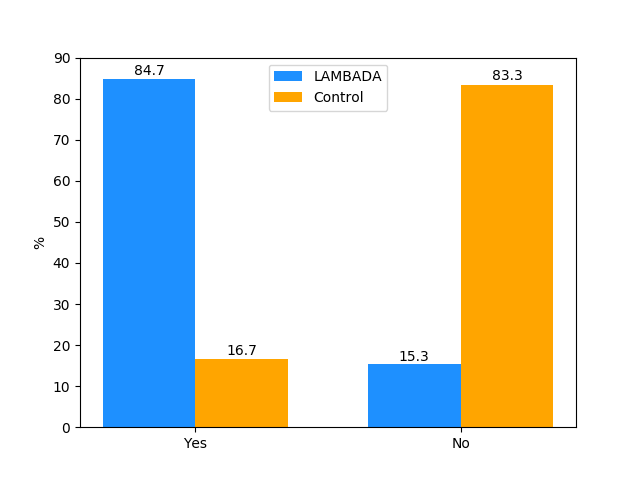
\includegraphics[scale=0.53]{lambadaContext}
	\captionof{figure}{Percentage of passages that contain the target word in the context.}
	\label{fig:lambadaContext}
\end{figure}

In 84.7 \% of the LAMBADA items the target word (or its lemma, extracted with \texttt{nltk}'s WordNetLemmatizer) is mentioned in the context, compared to the 15.3 \% for the control set. Furthermore, we can study the mention distance (understood as the number of words between the target word and its mention) distribution for LAMBADA. As illustrated in \autoref{fig:lambadaDistance}, 73 \% of the mentions are at a distance of more than 30 words (LAMBADA passages feature an average length of 75 words). This is specially important as many of the publicly available RNNLMs implementations are trained with TBPTT using $k_2$ somewhere between 20 and 35.
 
\begin{figure}[H]
	\centering
	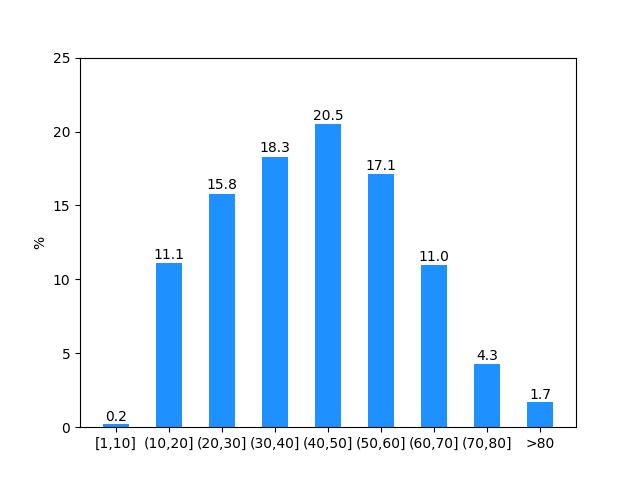
\includegraphics[scale=0.53]{lambadaDistance}
	\captionof{figure}{Distribution of average distance between the target word and a previous mention in LAMBADA.}
	\label{fig:lambadaDistance}
\end{figure}

Moreover, it is also interesting to study the part of speech (PoS) tag distribution of the target words (also extracted with \texttt{nltk}'s default PoS tagger). As shown in \autoref{fig:lambadaPos}, the largest portion of target words are proper nouns (48.1\%) followed by common nouns (37\%) and, far-off, verbs (7.7\%). By comparing with control's PoS distribution, it is clear that proper nouns are over-represented in LAMBADA while the rest of the categories are downplayed.

\begin{figure}[H]
	\centering
	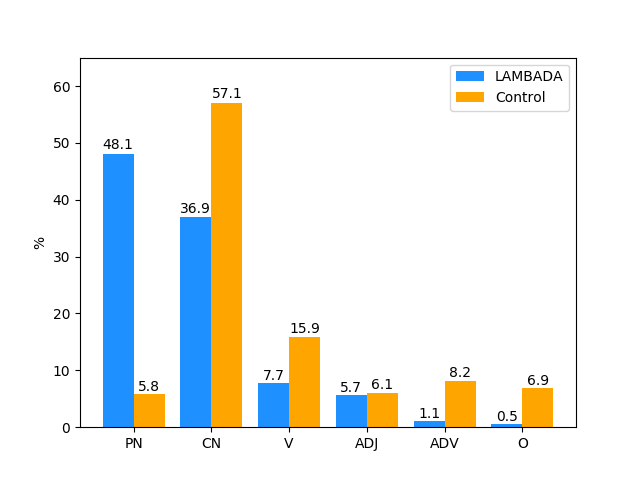
\includegraphics[scale=0.53]{lambadaPos}
	\captionof{figure}{Target words' PoS distribution (PN=proper noun, CN=common noun, V=verb, ADJ=adjective, ADV=adverb, O=other).}
	\label{fig:lambadaPos}
\end{figure}

\begin{figure}[H]
	\centering
	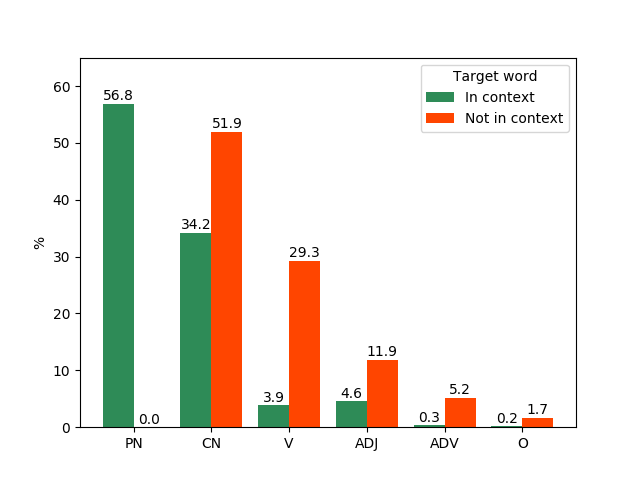
\includegraphics[scale=0.53]{lambadaPosAndContext}
	\captionof{figure}{LAMBADA target words' PoS distribution splitted depending on whether it is mentioned in the context.}
	\label{fig:lambadaPosAndContext}
\end{figure}

The authors argue that the reason for this bias is the fact that proper nouns are favored by the specific setup. Namely, in many cases the context clearly demands a referential expression and the constraint of predicting a single word excludes other possibilities such as noun phrases with articles. This hypothesis seems to be confirmed by \autoref{fig:lambadaPosAndContext}, which shows the PoS distribution for LAMBADA split depending on whether the target word appears in the context. It can be seen that explicit mention in the preceding discourse context is critical for proper nouns (when the target word does not previously appear in the passage, none of them are proper nouns), while the other categories can often be guessed without having been explicitly introduced.

To sum up, we can conclude that LAMBADA does indeed put to the test language models' capabilities to exploit \textbf{long-range dependencies}. Besides, it is also important to note the bias towards proper nouns present in the dataset. Proper nouns are used to refer to unique entities (e.g. the name of a specific character in a book) and due to their nature, they are \textbf{rare words} (when compared to the rest of the training corpus). We will describe this phenomena in detail in the next section.

\section{The Rare Word Problem}
\label{sec:problemRare}

As we saw in \autoref{chapter:nlm}, a common approach followed by recent neural language models is to use a softmax output layer where each of the dimensions corresponds to a word in a predefined vocabulary.

This approach has a fundamental problem, known as the \textit{rare word problem} \cite{merity2016pointer}. It is caused by some of the words in the vocabulary occurring much less frequently in the training set and thus, making the process of learning a good representation for them difficult. This in turn leads to poor generalization performance. 

\begin{figure}[H]
	\centering
	\begin{subfigure}{.5\textwidth}
		\centering
		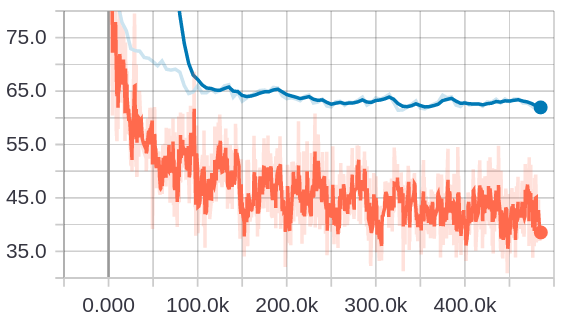
\includegraphics[scale=0.325]{perplexity_all}
		\caption{All words}
		\label{fig:perplexity_all}
	\end{subfigure}%
	\begin{subfigure}{.5\textwidth}
		\centering
		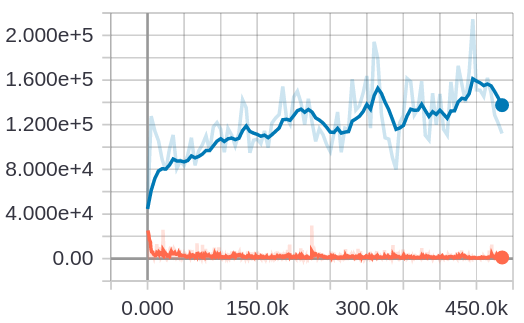
\includegraphics[scale=0.325]{perplexity_names}
		\caption{Only names}
		\label{fig:perplexity_names}
	\end{subfigure}
	\caption{Perplexity traces on LAMBADA for a vanilla LSTM (training trace is in orange and development, in blue).}
	\label{fig:perplexityRare}
\end{figure}

\autoref{fig:perplexityRare} illustrates a real example of this problem. \autoref{fig:perplexity_all} shows traces of average word perplexity over training batches and the development set for a vanilla LSTM language model trained on the LAMBADA training partition (more details in \autoref{chapter:experiments}). If we now focus on just rare words (in this specific example, character names), we can see in \autoref{fig:perplexity_names} that the model is clearly overfitting on this subset of words. Intrinsically, rare words constitute a small fraction of the corpus and hence, their effect is averaged out when taking into account all words.

These results suggest that in general existing neural language models have the fundamental problem of failing to handle rare words. Despite the limited effect on the overall perplexity, the rare word problem is a significant issue for language models. Rare words are of primary interest in many applications that rely on knowledge-extraction, such as question-answering or reading comprehension.

\section{RNN Regularization}
\label{sec:rnnRegularization}

To end this chapter, we will describe in detail several recent efforts for effectively regularizing and avoiding overfitting in recurrent neural networks:

\subsection{Dropout}

Neural networks are very expressive models that can learn very complicated input-output mappings which may in turn lead to overfitting. Ensemble methods such as model averaging (where we average the outputs of several estimators that have been trained independently) are known to nearly always improve their single base estimators and have a regularization effect as the variance of the resulting model is reduced. However, the idea of averaging the outputs of many separately trained neural networks is prohibitively expensive. 

Dropout is an extremely effective and simple regularization technique introduced in \cite{srivastava14a}. It is implemented by only keeping a neuron active with some probability $p$ (a hyperparameter), or setting it to zero otherwise. If we consider a network with $n$ units, the application of dropout can generate $2^n$ different possible ``reduced'' networks (all of them sharing the same weights). In words of the authors, \textit{``training a neural network with dropout provides a way of approximately training a collection of $2^n$ thinned networks with extensive weight sharing, where actually each thinned network gets trained very rarely, if at all''}.

At test time, it is not feasible to explicitly average the predictions from exponentially many models. However, a very simple approximate averaging method is then used: no dropout is applied while testing and all weights are scaled by $p$ (same probability as used during training). This has the goal of ensuring that for any unit, the expected output (under the dropout distribution used in training time) is the same as the actual output at test time. Given a unit's output $y$, its expected value is $\mathbb{E}[y]=py+(1-p)0=py$.

In practice, we employ a variant known as \textbf{``inverted dropout''} where the units that are kept are also scaled by $1/p$. This has the very appealing property of not requiring any additional operations during test time.

One of the first successful attempts at applying dropout for regularizing RNNs was described in \cite{zaremba2014recurrent}. The authors claim that dropout should only be applied to non-recurrent connections (namely, input and output units) by sampling a different dropout mask at each time step. Therefore it is ensured that information is only corrupted $L+1$ times (being $L$ the number of layers of the RNN), as exemplified in \autoref{fig:flowDropout}. In this way, the method can benefit from dropout regularization without sacrificing the valuable memorization ability of RNNs.

\begin{figure}[H]
	\centering
	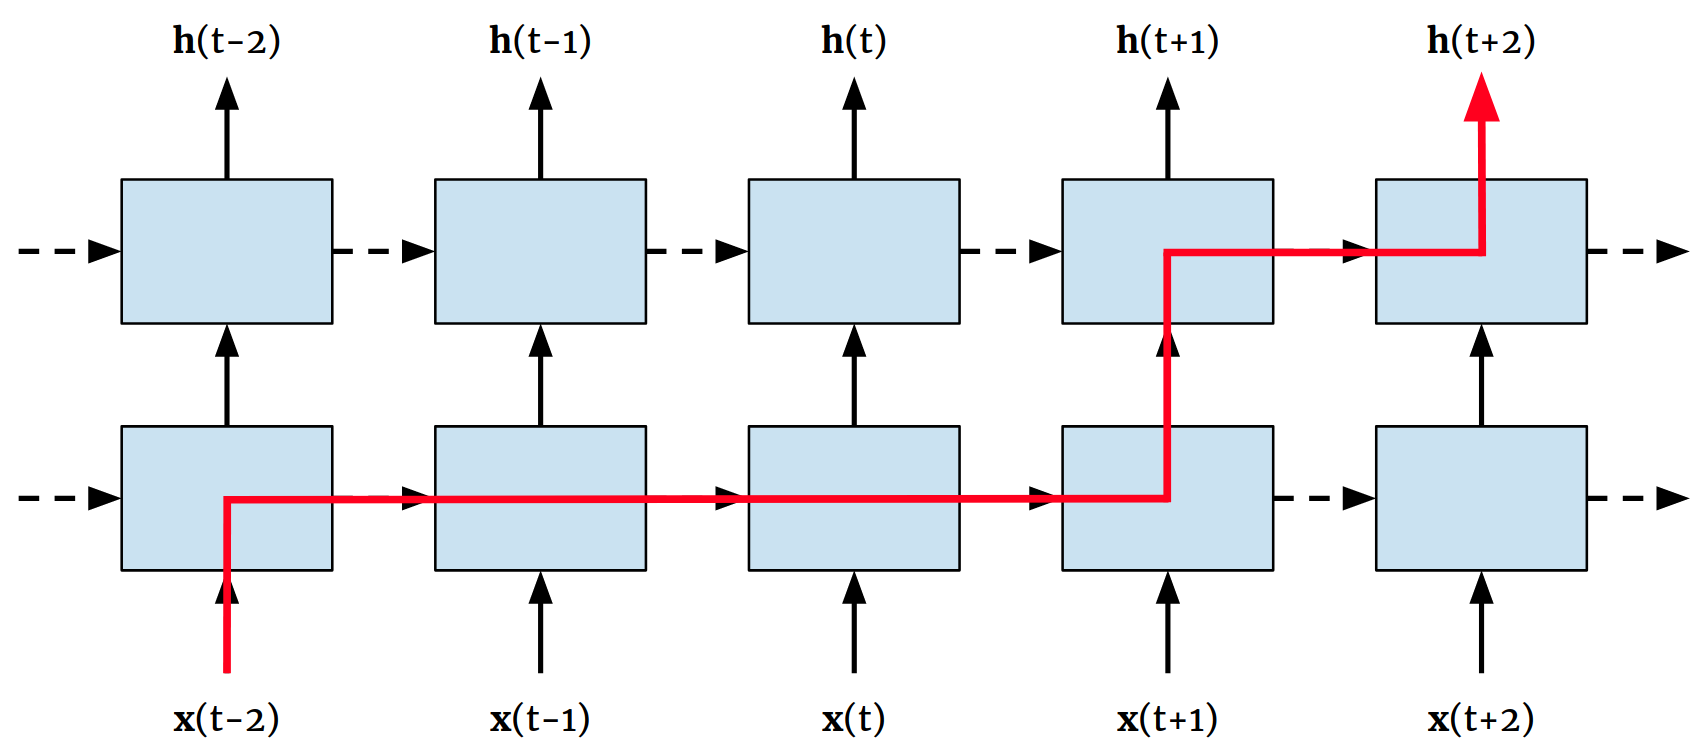
\includegraphics[scale=0.2]{flowDropout}
	\captionof{figure}{Example of information flow in a multilayer RNN with dropout (only applied at connections denoted with a solid arrow).}
	\label{fig:flowDropout}
\end{figure}

\subsection{Variational Dropout}

Following previous results at the intersection of Bayesian research and deep learning, \cite{gal2016theoretically} proposes a new dropout variant theoretically grounded on the results arisen from the application of approximate variational inference to probabilistic Bayesian RNNs. 

Given a training dataset consisting of the sequence of inputs $\mathbf{X}=\{\mathbf{x}(1),\\\cdots,\mathbf{x}(N)\}$ and outputs $\mathbf{Y}=\{\mathbf{y}(1),\cdots,\mathbf{y}(N)\}$, Bayesian parametric regression aims to infer the parameters $W$ of a function $\mathbf{y}=\mathbf{f}^W(\mathbf{x})$ (in our derivation, $\mathbf{f}^W(\cdot)$ is a neural network and $W$ are its weight matrices). Following the Bayesian methodology, we place a prior distribution $p(W)$ over the weights (often a standard multivariate Gaussian) and define a likelihood distribution $p(\mathbf{y} |\mathbf{x}, W)$ (usually assumed to be a softmax likelihood) and a posterior distribution $p(W | \mathbf{X}, \mathbf{Y})$ given the observed dataset.

For a new input point $\mathbf{x^*}$, an output can then be predicted as shown in \autoref{eq:post}. However this is not feasible in practice as the posterior is not tractable in general. 

\begin{equation} \label{eq:post}
\begin{gathered}
	p(W | \mathbf{X}, \mathbf{Y}) = \frac{ p(\mathbf{Y} | \mathbf{X}, W) p(W) }{ p( \mathbf{Y} ) } \\
	p(\mathbf{y^*} | \mathbf{x^*}, \mathbf{X}, \mathbf{Y}) = \int p(\mathbf{y^*} | \mathbf{x^*}, W) p(W | \mathbf{X}, \mathbf{Y}) dW
\end{gathered}
\end{equation}

To work around this problem, variational inference can be used to approximate the posterior with a variational distribution $q(W)$ and then
minimize the Kullback–Leibler (KL) divergence between the approximating distribution and the full posterior (\autoref{eq:varInference}). 

\begin{equation} \label{eq:varInference}
\begin{gathered}
	\mathcal{L}=\text{KL}(q(W)||p(W | \mathbf{X}, \mathbf{Y})) \propto - \int q(W) \log(p(\mathbf{Y} | \mathbf{X}, W))dW + \text{KL}(q(W)||p(W))\\
	= - \sum_{i=1}^{N} \int q(W) \log(p(\mathbf{y}(i) | \mathbf{f}^W(\mathbf{x}(i))))dW + \text{KL}(q(W)||p(W))
\end{gathered}
\end{equation}

Going now to the specifics of RNNs, we can further define each input point $\mathbf{x}$ to be a sequence $[\mathbf{x}(1),\cdots,\mathbf{x}(T)]$ of length $T$, the model output as $\mathbf{f_y}^W(\cdot)$ and the recurrent cell function as $\mathbf{f_h}^W(\cdot)$ (both of them with their respective weight matrices). Then the integral from \autoref{eq:varInference} can be rewritten as:

\begin{equation} \label{eq:approximation}
\begin{gathered}
	\int q(W) \log(p(\mathbf{y} | \mathbf{f_y}^W(\mathbf{h}(T))))dW \\ 
	= \int q(W) \log(p(\mathbf{y} | \mathbf{f_y}^W(\mathbf{f_h}^W(\mathbf{x}(T),\mathbf{h}(T-1)))))dW \\
	= \int q(W) \log(p(\mathbf{y} | \mathbf{f_y}^W(\mathbf{f_h}^W(\mathbf{x}(T),\mathbf{f_h}^W(\ldots\mathbf{f_h}^W(\mathbf{x}(1),\mathbf{h}(0)\ldots)))))dW \\
	\stackrel{*}{\approx} \log(p(\mathbf{y}| \mathbf{f_y}^{\hat{W}}(\mathbf{f_h}^{\hat{W}}(\mathbf{x}(T),\mathbf{f_h}^{\hat{W}}(\ldots\mathbf{f_h}^{\hat{W}}(\mathbf{x}(1),\mathbf{h}(0)\ldots))))) \, \text{with} \, \hat{W} \sim q(W)
\end{gathered}
\end{equation}

where $*$ means that the integral is approximated with Monte Carlo (MC) integration with a single sample.

Then the minimization objective can be formulated as:

\begin{equation} \label{eq:finalVarLoss}
\begin{gathered}
	\mathcal{L} \approx - \sum_{i=1}^{N} \log(p(\mathbf{y}(i) | \mathbf{f_y}^{\hat{W}}(\mathbf{f_h}^{\hat{W_i}}(\mathbf{x}(i,T),\mathbf{f_h}^{\hat{W_i}}(\ldots\mathbf{f_h}^{\hat{W_i}}(\mathbf{x}(i,1),\mathbf{h}(0)\ldots))))) \\ 
	+ \text{KL}(q(W)||p(W))
\end{gathered}
\end{equation}

It is important to note in \autoref{eq:finalVarLoss} that new weights are sampled for each point in the dataset. However, the weights are kept the same for all the time steps $t<T$ of every input sequence. Finally, the approximating distribution $q(W)$ is defined to factorize over the different weight matrices and their rows $\mathbf{w_k}$ as:

\begin{equation} \label{eq:approxPost}
	q(\mathbf{w_k})=p\mathcal{N}(\mathbf{m_k},\sigma^2\mathbf{I})+(1-p)\mathcal{N}(\mathbf{0},\sigma^2\mathbf{I})
\end{equation}

where $\mathbf{m_k}$ is a vector of variational parameters.

First we can see in \autoref{eq:approxPost} that sampling from $q(W)$ is identical to applying dropout on the weight matrices. Second, implementing the described approximate inference procedure is equivalent to performing dropout in RNNs with the same network units dropped at each time step, randomly dropping inputs, outputs, and recurrent connections. \autoref{fig:compareDropout} graphically illustrates the main differences of this method with respect to the one introduced in the previous section.

\begin{figure}[H]
	\centering
	\begin{subfigure}{.5\textwidth}
		\centering
		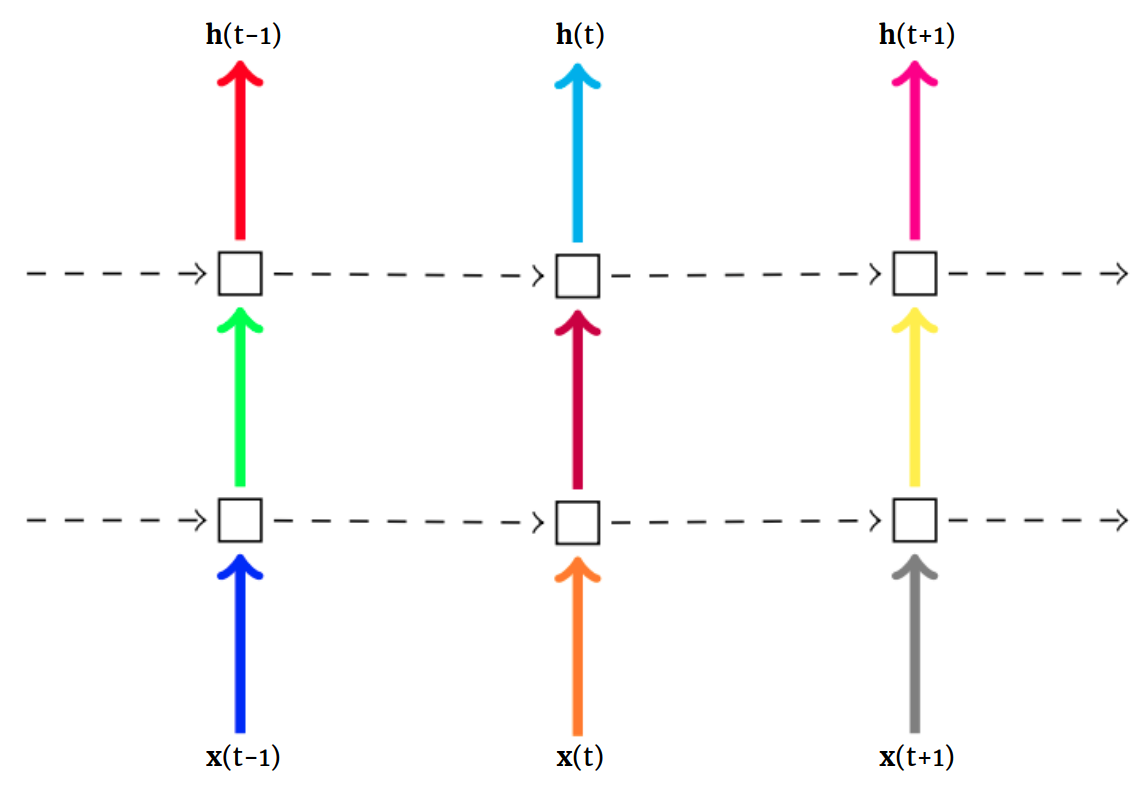
\includegraphics[scale=0.16]{dropout}
		\caption{``Naive''}
		\label{fig:dropout}
	\end{subfigure}%
	\begin{subfigure}{.5\textwidth}
		\centering
		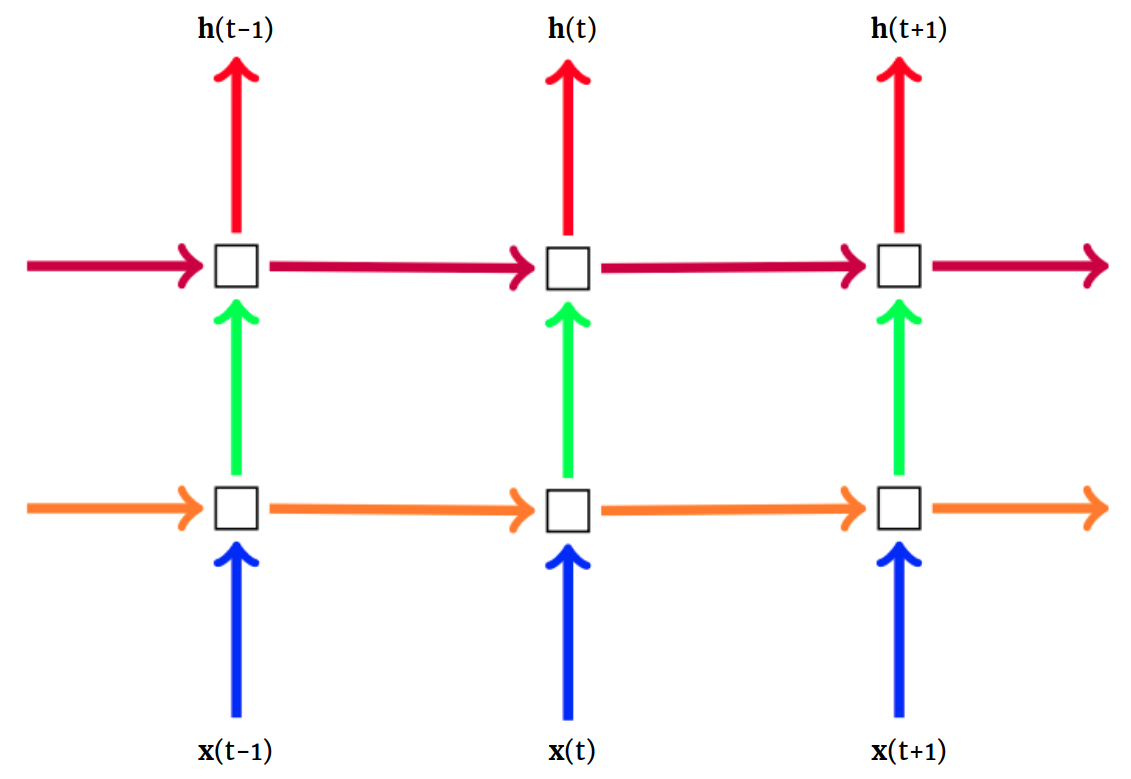
\includegraphics[scale=0.16]{varDropout}
		\caption{Variational}
		\label{fig:varDropout}
	\end{subfigure}
	\caption{Comparison of dropout techniques (only applied at connections denoted with a solid arrow, with different colors representing different masks) \cite{gal2016theoretically}.}
	\label{fig:compareDropout}
\end{figure}

\subsection{Zoneout}

An alternative regularization method that only applies to the recurrent connections of an RNN was introduced in \cite{krueger2016zoneout}. Rather than setting a unit's activation to 0 with probability $1-p$ as in dropout, zoneout replaces the unit's activation with its value from the previous time step. We can see in \autoref{eq:zoneout} what is the formulation of zoneout for the LSTM cell:

\begin{equation} \label{eq:zoneout}
	\begin{gathered}
		\mathbf{c}(t) = \mathbf{d_c}(t)\odot\mathbf{c}(t-1) + (1-\mathbf{d_c}(t))\odot(\mathbf{f}(t) \odot \mathbf{c}(t-1) + \mathbf{i}(t) \odot \mathbf{\tilde{c}}(t)) \\
		\mathbf{h}(t) = \mathbf{d_h}(t)\odot\mathbf{h}(t-1) \\ 
		+ (1-\mathbf{d_h}(t))\odot (\mathbf{o}(t) \odot \tanh(\mathbf{f}(t) \odot \mathbf{c}(t-1) + \mathbf{i}(t) \odot \mathbf{\tilde{c}}(t)))
	\end{gathered}
\end{equation}

where $\mathbf{d_c}(t)$ and $\mathbf{d_h}(t)$ are Bernoulli random vectors.

It as argued by the authors that compared with dropout, zoneout is appealing because it preserves information flow forwards and backwards through the network. This in turn seems to help with the vanishing gradient problem, as shown by their experimental results.

\subsection{Weight Dropout}

The recent work described in \cite{merity2017regularizing} opts for applying DropConnect \cite{wan2013regularization} on the recurrent connections of a recurrent cell. For an LSTM, it is implemented by applying on the recurrent weight matrices ($U_f,U_i,U_o,U_f$ from \autoref{eq:lstmcell}) a Bernoulli mask  sampled before each forward-backward pass. It is similar to variational dropout in the sense that the same mask is reused over multiple time steps. However, by working directly on the weight matrices, ``weight dropout'' doesn't need to modify the formulation of the cell and is amenable to be used with highly optimized black box implementations.
\chapter{Experiments and Results}

experiments... \todo{Finish experiments and results}

\begin{equation}
\begin{split}
  \mathcal{L}=-\sum_{n} \log(P(name|h_t)P(w_t|h_t, name) + (1-P(name|h_t))P(w_t|h_t, notName)) \\
   + \lambda(y_{name}\log(P(name|h_t)) + (1 - y_{name})\log(1-P(name|h_t))
\end{split}
\end{equation}

\begin{table}[]
	\centering
	\begin{tabular}{cc|c|c|c|c|}
		\cline{3-6}
		\multicolumn{1}{l}{}                                                    & \multicolumn{1}{l|}{}   & \multicolumn{2}{c|}{All} & \multicolumn{2}{c|}{Names} \\ \cline{3-6} 
		&                         & Train       & Dev        & Train        & Dev         \\ \hline
		\multicolumn{1}{|c|}{\multirow{2}{*}{Basic}}                            & Baseline                & 42.5        & 61.5       & 1000         & 130K        \\ \cline{2-6} 
		\multicolumn{1}{|c|}{}                                                  & Mixture ($\lambda=100$) & 55          & 69         & 4000         & 120K        \\ \hline
		\multicolumn{1}{|c|}{\multirow{2}{*}{Input dropout}}                    & Baseline                & 52.5        & 63         & 2000         & 140K        \\ \cline{2-6} 
		\multicolumn{1}{|c|}{}                                                  & Mixture ($\lambda=100$) & 65          & 72         & 8000         & 120K        \\ \hline
		\multicolumn{1}{|c|}{\multirow{2}{*}{State dropout}}                    & Baseline                & 48          & 62.5       & 1000         & 120K        \\ \cline{2-6} 
		\multicolumn{1}{|c|}{}                                                  & Mixture ($\lambda=100$) & 62.5        & 73         & 6000         & 120K        \\ \hline
		\multicolumn{1}{|c|}{\multirow{2}{*}{Output dropout}}                   & Baseline                & 62.5        & 65         & 5000         & 150K        \\ \cline{2-6} 
		\multicolumn{1}{|c|}{}                                                  & Mixture ($\lambda=100$) & 80          & 73         & 20K          & 80K         \\ \hline
		\multicolumn{1}{|c|}{\multirow{2}{*}{L2 regularization ($\beta=0.01$)}} & Baseline                & 100         & 125        & 10K          & 400K        \\ \cline{2-6} 
		\multicolumn{1}{|c|}{}                                                  & Mixture ($\lambda=100$) & 107.5       & 119        & 8000         & 120K        \\ \hline
	\end{tabular}
	\caption{Perplexity}
	\label{my-label}
\end{table}
\chapter{Conclusion}

\section{Achieved Results}
\label{sec:achieved}

\section{Future Work}
\label{sec:futureWork}

Extend neural language models to handle OOV words ?



\backmatter

\nocite{*} % REMOVE AT THE END (OR NOT)
\bibliographystyle{unsrt}
\bibliography{refs}
\clearpage\thispagestyle{empty}\null\newpage

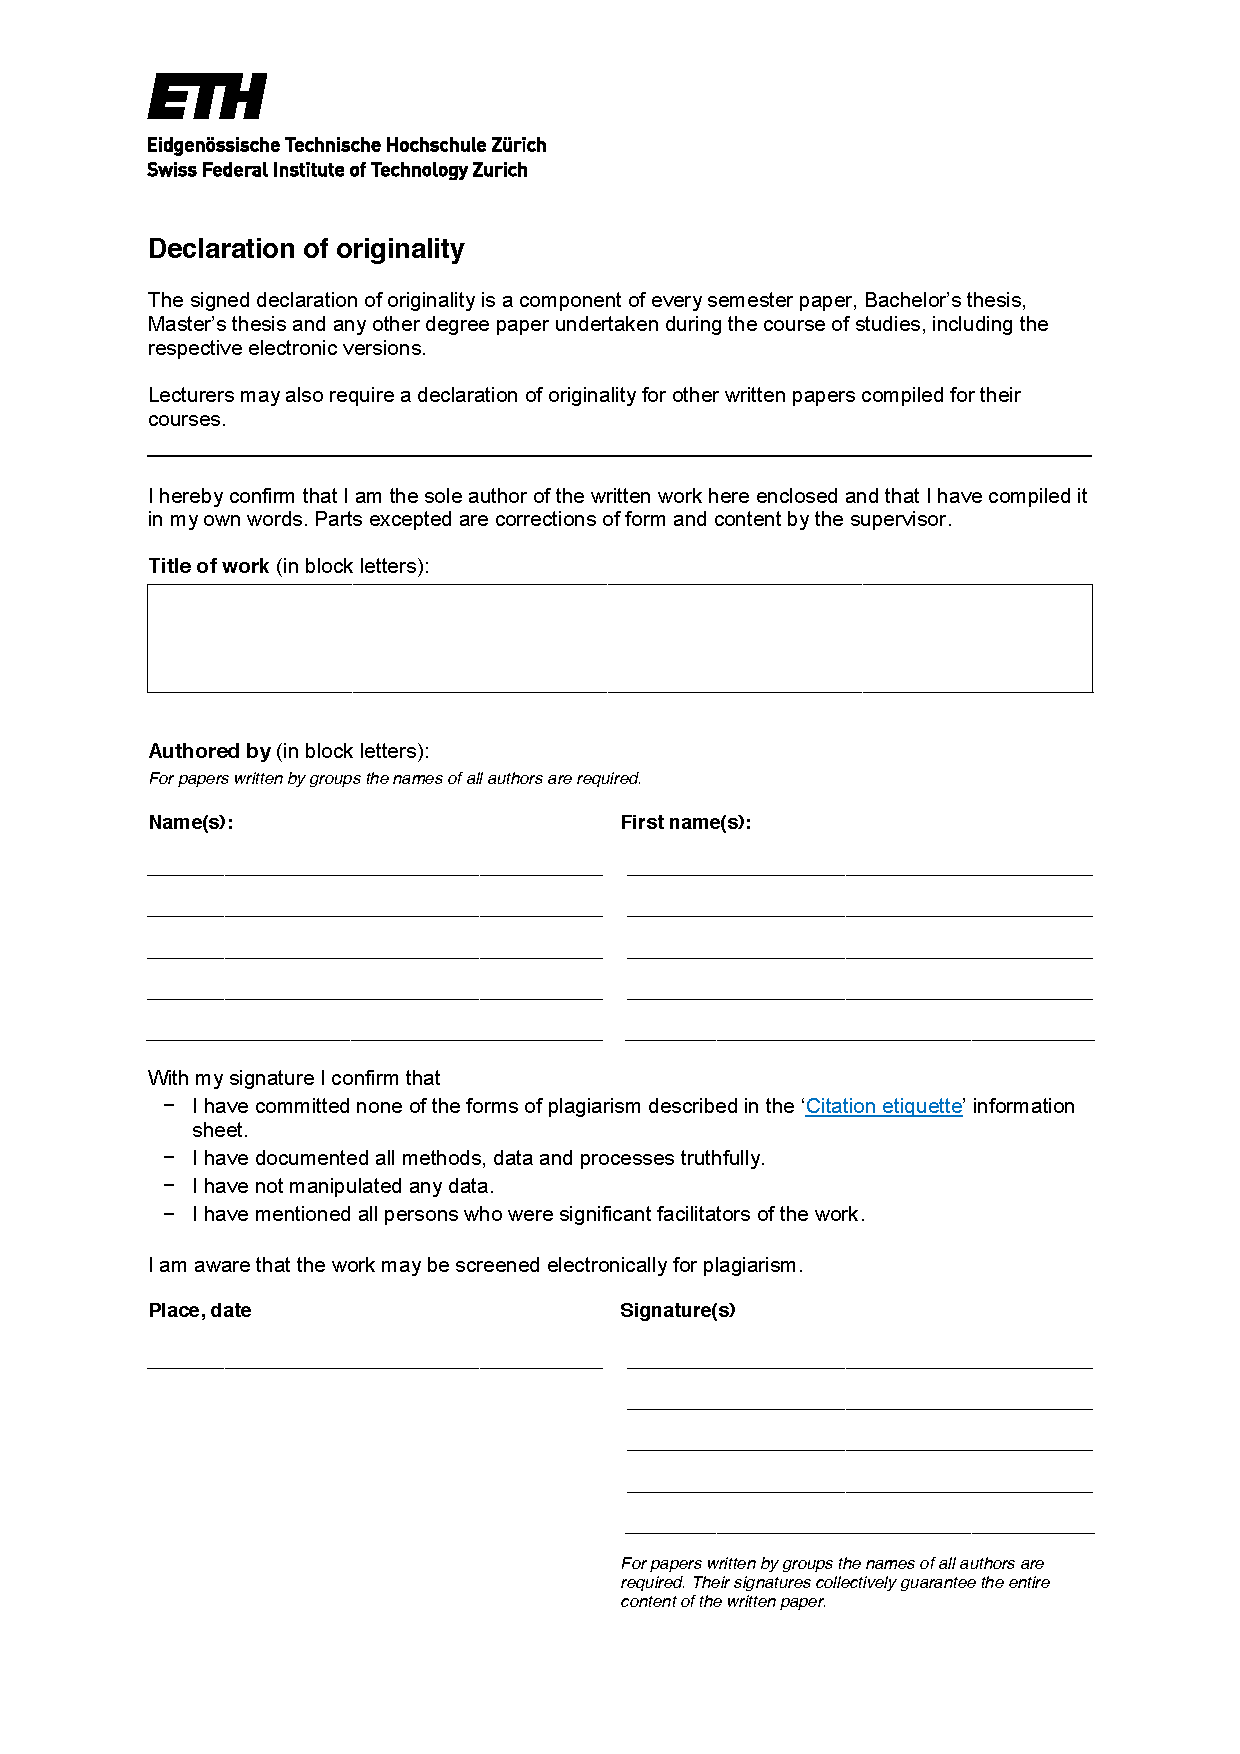
\includepdf[pages={-}]{declaration-originality.pdf}

\end{document}